\section{Интеграция решения по аутентификации пользователей в корпоративных
информационных системах с использованием ПЦКД}

Решение задачи интеграции клиентского решения по аутентификации и авторизации на
основе ПЦКД с корпоративными
информационными системами требует создания модуля адаптации, реализующего
непосредственное взаимодействие с интерфейсами информационных систем и имеющего
четкий протокол методов и параметров взаимодействия. Одним из возможных решений,
обеспечивающим универсальность и независимость клиентской части от архитектуры
самих корпоративных ИС является технология RPC (Remote Procedure Call или вызов
удаленных процедур).

\subsection{Технология RPC}
 
Идея вызова удаленных процедур состоит в расширении хорошо
известного и понятного механизма передачи управления и данных внутри программы,
выполняющейся на одной машине, на передачу управления и данных через сеть.
Средства удаленного вызова процедур предназначены для облегчения организации
распределенных вычислений. Наибольшая эффективность использования RPC
достигается в тех приложениях, в которых существует интерактивная связь между
удаленными компонентами с небольшим временем ответов и относительно малым
количеством передаваемых данных.

Характерными чертами вызова локальных процедур являются:
\begin{itemize}
  \item Асимметричность, то есть одна из взаимодействующих сторон является
инициатором;
\item Синхронность, то есть выполнение вызывающей процедуры при
останавливается с момента выдачи запроса и возобновляется только после возврата
из вызываемой процедуры.
\end{itemize}

Реализация удаленных вызовов существенно сложнее реализации вызовов локальных
процедур. Поскольку вызывающая и вызываемая процедуры выполняются на разных
машинах, то они имеют разные адресные пространства, и это создает проблемы при
передаче параметров и результатов, особенно если машины не идентичны. Так как
RPC не может рассчитывать на разделяемую память, то это означает, что параметры
RPC не должны содержать указателей на ячейки нестековой памяти и что значения
параметров должны копироваться с одного компьютера на другой. Следующим отличием
RPC от локального вызова является то, что он обязательно использует нижележащую
систему связи, однако это не должно быть явно видно ни в определении процедур,
ни в самих процедурах. Удаленность вносит дополнительные проблемы. Выполнение
вызывающей программы и вызываемой локальной процедуры в одной машине реализуется
в рамках единого процесса. Но в реализации RPC участвуют как минимум два
процесса -- по одному в каждой машине.~\cite{rpc}

К преимуществам технологии RPC
можно отнести следующее:
\begin{itemize}
  \item высокий уровень скрытия реализации процедур;
  \item широкие возможности для
встраивания различных подсистем;
\item гибкие возможности внесения изменений в
функционирование системы.
\end{itemize}

Взаимодействие программных компонентов при выполнении удаленного вызова
процедуры иллюстрируется рисунком~\ref{ris:3.4.1}. 

\begin{figure}[h!]
\center{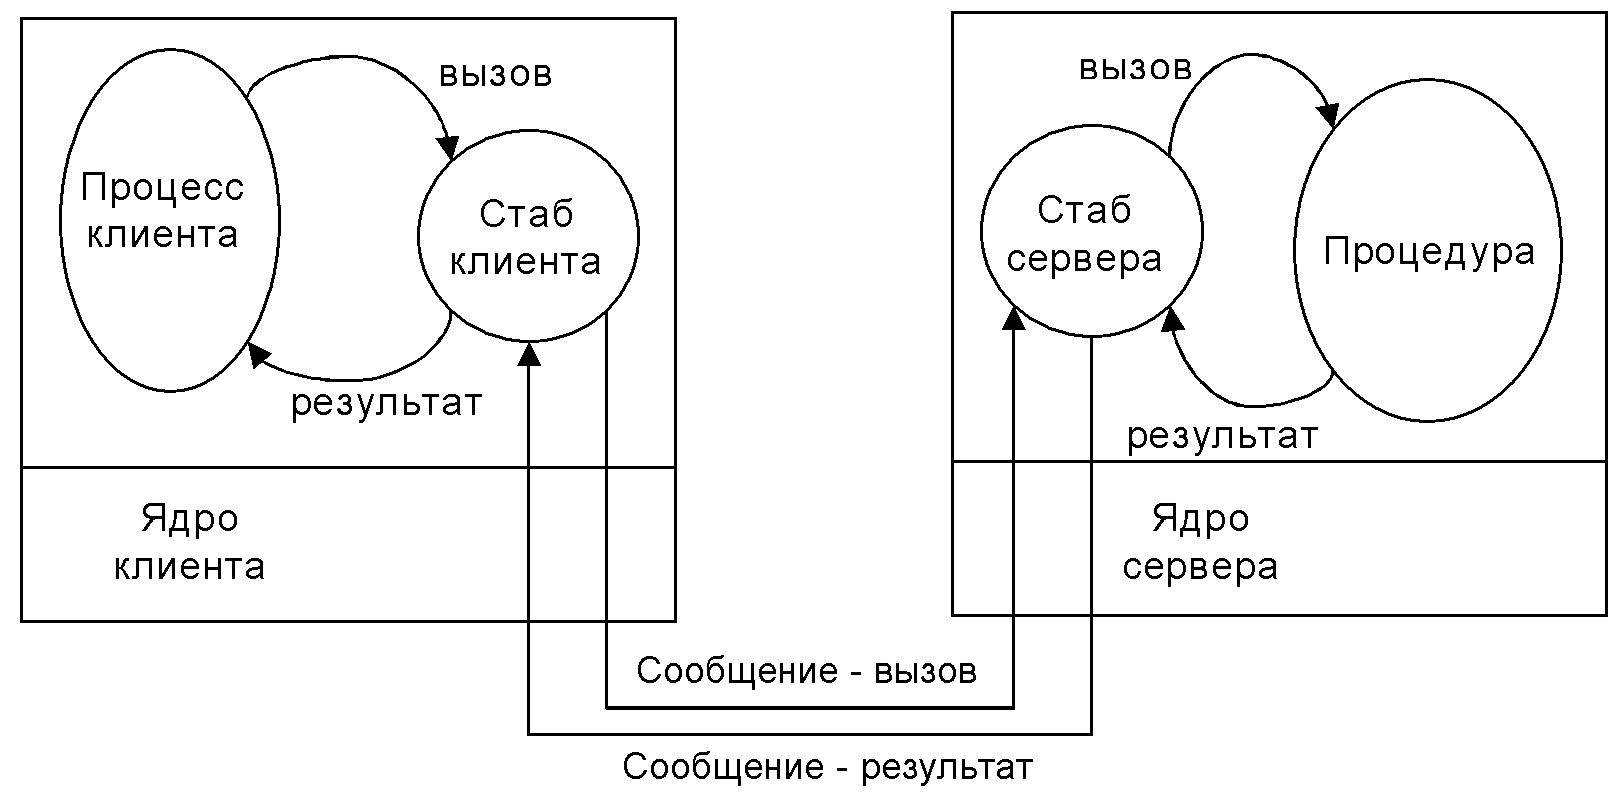
\includegraphics[width=1\linewidth]{3-4-1}}
\caption{Remote Procedure Call}
\label{ris:3.4.1}
\end{figure}

После того, как клиентский стаб (stub -
заглушка) был вызван программой-клиентом, его первой задачей является заполнение
буфера отправляемым сообщением. В некоторых системах клиентский стаб имеет
единственный буфер фиксированной длины, заполняемый каждый раз с самого начала
при поступлении каждого нового запроса. В других системах буфер сообщения
представляет собой пул буферов для отдельных полей сообщения, причем некоторые
из этих буферов уже заполнены. Этот метод особенно подходит для тех случаев,
когда пакет имеет формат, состоящий из большого числа полей, но значения многих
из этих полей не меняются от вызова к вызову.
Затем параметры должны быть преобразованы в соответствующий формат и вставлены в
буфер сообщения. К этому моменту сообщение готово к передаче, поэтому
выполняется прерывание по вызову ядра.

Когда ядро получает управление, оно переключает контексты, сохраняет регистры
процессора и карту памяти (дескрипторы страниц), устанавливает новую карту
памяти, которая будет использоваться для работы в режиме ядра. Поскольку
контексты ядра и пользователя различаются, ядро должно точно скопировать
сообщение в свое собственное адресное пространство так, чтобы иметь к нему
доступ, запомнить адрес назначения (а, возможно, и другие поля заголовка), а
также оно должно передать его сетевому интерфейсу. На этом завершается работа на
клиентской стороне. Включается таймер передачи, и ядро может либо выполнять
циклический опрос наличия ответа, либо передать управление планировщику, который
выберет какой-либо другой процесс на выполнение. В первом случае ускоряется
выполнение запроса, но отсутствует мультипрограммирование.

На стороне сервера поступающие биты помещаются принимающей аппаратурой либо во
встроенный буфер, либо в оперативную память. Когда вся информация будет
получена, генерируется прерывание. Обработчик прерывания проверяет правильность
данных пакета и определяет, какому стабу следует их передать. Если ни один из
стабов не ожидает этот пакет, обработчик должен либо поместить его в буфер, либо
вообще отказаться от него. Если имеется ожидающий стаб, то сообщение копируется
ему. Наконец, выполняется переключение контекстов, в результате чего
восстанавливаются регистры и карта памяти, принимая те значения, которые они
имели в момент, когда стаб сделал вызов receive.

Теперь начинает работу серверный стаб. Он распаковывает параметры и помещает их
соответствующим образом в стек. Когда все готово, выполняется вызов сервера.
После выполнения процедуры сервер передает результаты клиенту. Для этого
выполняются все описанные выше этапы, только в обратном порядке.

\subsection{Общая схема интеграции модулей ПЦКД в корпоративные ИС}

Рассмотрев специфику взаимодействия программных компонентов системы
аутентификации с применением ПЦУД, была предложена схема (рисунок~\ref{ris:3.4.2})
интеграции клиентских программных компонентов в сервер доступа, используя технологию RPC.

\begin{figure}[h!]
\center{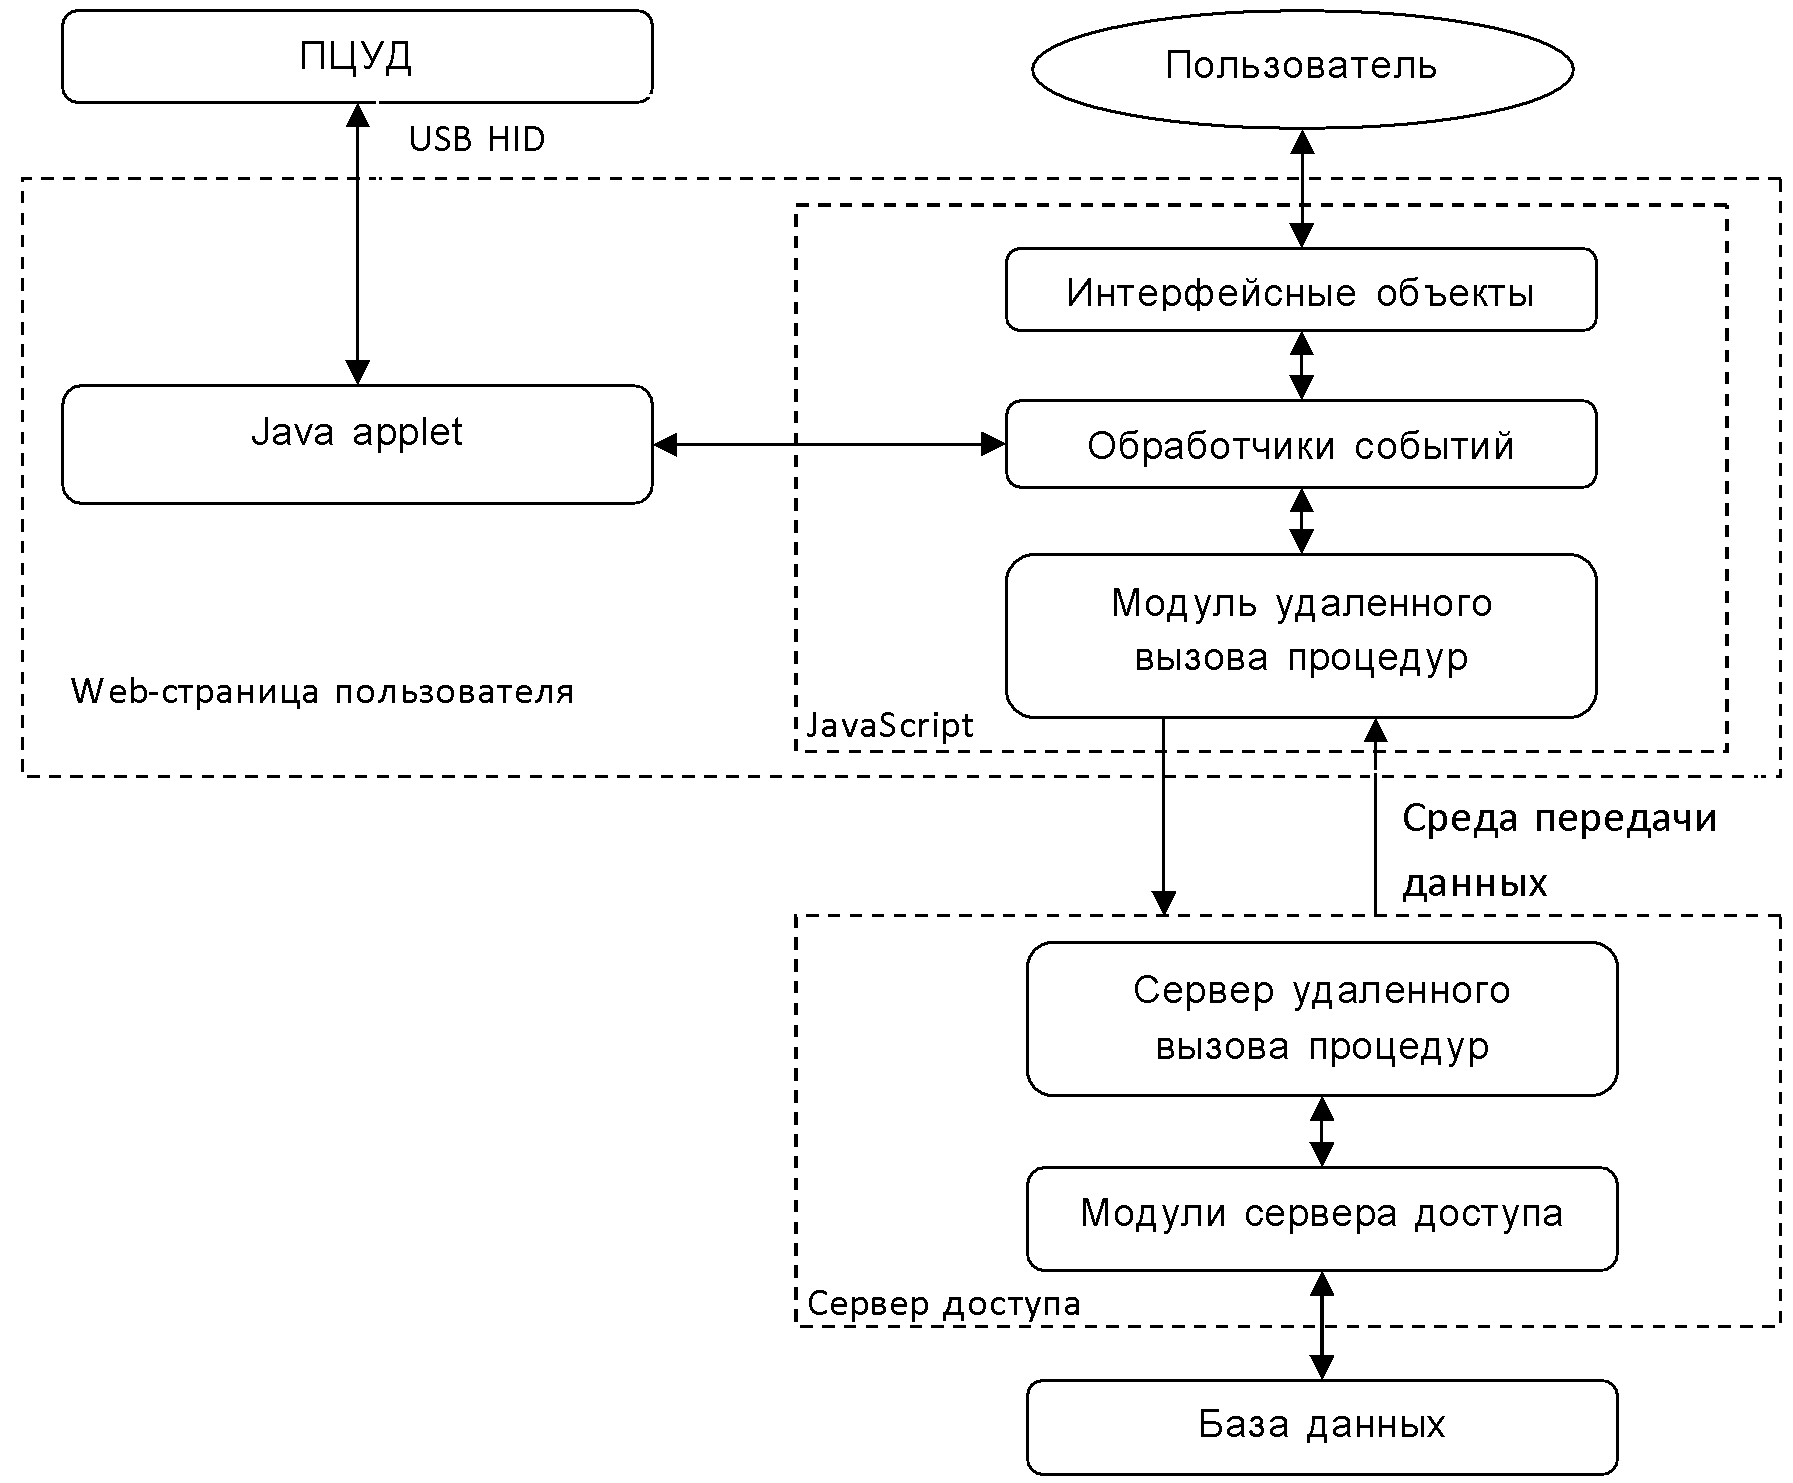
\includegraphics[width=1\linewidth]{3-4-2}}
\caption{Схема интеграции клиентского решения на основе ПЦКД с серверами
контроля доступа, используя технологию RPC}
\label{ris:3.4.2}
\end{figure} 

В соответствии с данной схемой можно выделить 4 сущности:
\begin{itemize}
  \item пользователь;
  \item web-страница пользователя;
  \item пользовательский ключ (ПЦКД);
  \item сервер доступа.
\end{itemize}

В Web-страницу встраивается Java-апплет и JavaScript. Java-апплет образует
магистраль передачи данных фиксированного формата в ПЦУД, подключенное к ПК по
интерфейсу USB-HID. JavaScript имеет описание и заголовки удаленных процедур,
физически размещенных на сервере доступа. По имеющимся заголовкам JS может
осуществлять удаленный вызов процедур, а так же передавать параметры и
обрабатывать результат. Для инициирования выполнения конкретной процедуры со
стороны пользователя, существуют интерфейсные объекты (кнопки, поля для ввода и
т.п.) и связанные с ними обработчики событий.
При появлении новой функции на сервере, достаточно определить интерфейсный
объект и привязать к нему обработчик события, после чего пользователь сможет
вызвать необходимую процедуру.
Наличие или отсутствие интерфейсных объектов может регулировать уровень доступа
на основе списка прав. Необходимый набор интерфейсных объектов описывает тот или
иной уровень прав доступа в соответствии с разрешениями для данного
пользователя.~\cite{art_rpc}

\subsection{Реализация механизма RPC}

При реализации механизма удаленного вызова процедур применительно к системе
аутентификации пользователей в сети корпоративных порталов с использованием
ПЦУД, было предложено задействовать одно из стандартных средств -- SimpleAjax
(SAJAX).

Sajax представляет собой инструмент с открытым исходным кодом, чтобы сделать
программирование веб-сайтов с помощью платформы Ajax как можно проще. Sajax
делает это при помощи вызова PHP, Perl, ColdFusion, IO, LUA, Ruby или Python
функций с помощью JavaScript без обновления web-страницы.~\cite{sajax} По факту
SimpleAjax выполняет асинхронные HTTP запросы (GET или POST) к удаленному
серверу передавая в качестве параметров заголовки процедур, предварительно
упакованных в формат XML. Общий формат вызываемой процедуры выглядит следующим
образом:

\begin{center}
  \textit{Call(procedure, [arguments], [callback]),} где 
 \end{center} 
 
 \textbf{procedure} --- обязательный параметр: строка, имя
 вызываемой процедуры;

\textbf{arguments} --- необязательный параметр: объект, аргументы вызываемой
процедуры;

\textbf{callback} --- необязательный параметр: функция принимающая объект,
реализует обработку ответа.

Содержимое данной процедуры преобразуется в формат XML, и далее передается на
сервер, где происходит обработка XML-объекта и выполнение удаленной процедуры.
При наличии возвращаемых параметров, они так же преобразуются в XML-объект,
который возвращается клиенту, где происходит его обработка.

Для выполнения заявленных функциональных требований, серверная часть подсистемы
должна реализовывать ряд функций~\ref{alg:2}, которые можно условно объединить в
следующие категории:
\begin{enumerate}
  \item Функции для управления пользователями и ключами (\textit{MakeUser,
  \\ ChangeKey});
  \item Функции для аутентификации пользователя (\textit{GetSoul, SetSession});
  \item Функции для выполнения документооборота \textit{(LoadFile, SignFile}).
\end{enumerate}

\begin{algorithm}[ht]
\floatname{algorithm}{Алгоритм}                
\caption{Описание функций клиентской части, физически размещенных на сервере
(RPC)}
\label{alg:2}     
\small                    
\begin{algorithmic}

\Procedure {MakeUser}{$username$} \Comment{Создание пользователя}

\Return{$massage$} \Comment{Шифрованное сообщение, содержащее ключ для ПЦКД}
\EndProcedure

\Procedure {ChangeKey}{$userid$} \Comment{Изменение ключа для
ПЦКД пользователя}

\Return{$massage$} \Comment{Шифрованное сообщение, содержащее ключ для ПЦКД}
\EndProcedure

\Procedure {GetSoul}{$void$} \Comment{Получение случайного
сообщения на сервере}

\Return{$Soul$} \Comment{Случайная последовательность}
\EndProcedure
  
\Procedure {SetSession}{$userid, signature$}  \Comment{Установка
сессии}

\Return{$CookieHash$} \Comment{CookieHash -- идентификатор сессии}
\EndProcedure

\Procedure {LoadFile}{$file, userid$}  \Comment{Загрузка файла на
сервер}
\EndProcedure

\Procedure {SignFile}{$filehash, signature$}  \Comment{Подписание
файла}
\EndProcedure

\end{algorithmic}
\end{algorithm}

Реализация механизма RPC, а также приведенных функций указана в
приложении~\ref{pril:C}.